\NewChapter{捏个怪兽吧!}


\quote{也许是因为我也想为幸福做一点什么吧!}{《鼠疫》}

《捏个怪兽吧!》是一款由腾讯 NExT Sutdios孵化的基于HTML5网页端的社交向UGC游戏,玩家可以通过做手工、捏橡皮泥的方式制作属于自己独一无二的怪兽,并与其它朋友的怪兽融合繁衍为新的怪兽。

在从19年末到22年末的三年多的时间里,我们都成了世界的孤岛。疫情的爆发让我们陷入了长期的封闭居家生活,与外界的交流仅限于虚拟的视频通话和文字信息。日子过得相似,便会过得很快,我们渐渐地迷失了自我,不知道该如何度过这漫长的时光。

如果说有什么好消息,那便是大家居家时学会的一些小爱好。我的家中便因此多了很多手工制品,在在这样的环境中,借腾讯NExT Studios Gameplus+ 跨界工作坊学习的机会,做出了《捏个怪兽吧!》试玩版。

在这段时间里,我也第一次领悟到游戏的跨界价值。世界很严苛,而游戏是一种媒介,它拥有完全改变人的能力,就像所有其它艺术和媒介能做到的一样。游戏应该被视作连结人与人、孤岛与孤岛的桥梁和纽带,游戏一定会让这个世界变得更好。好的游戏会让人变得更加温暖、更加坚韧。我希望《捏个怪兽吧!》能帮助人们在孤岛中创造出了属于自己的快乐。

\textbf{游戏原型目前在工作坊Final Critique中获得诸多好评,预计2023年第二季度上线推广。}

\begin{figure}[H]
\centering  %图片全局居中
\subfigure[Final Critique 老师创作的爱心]{
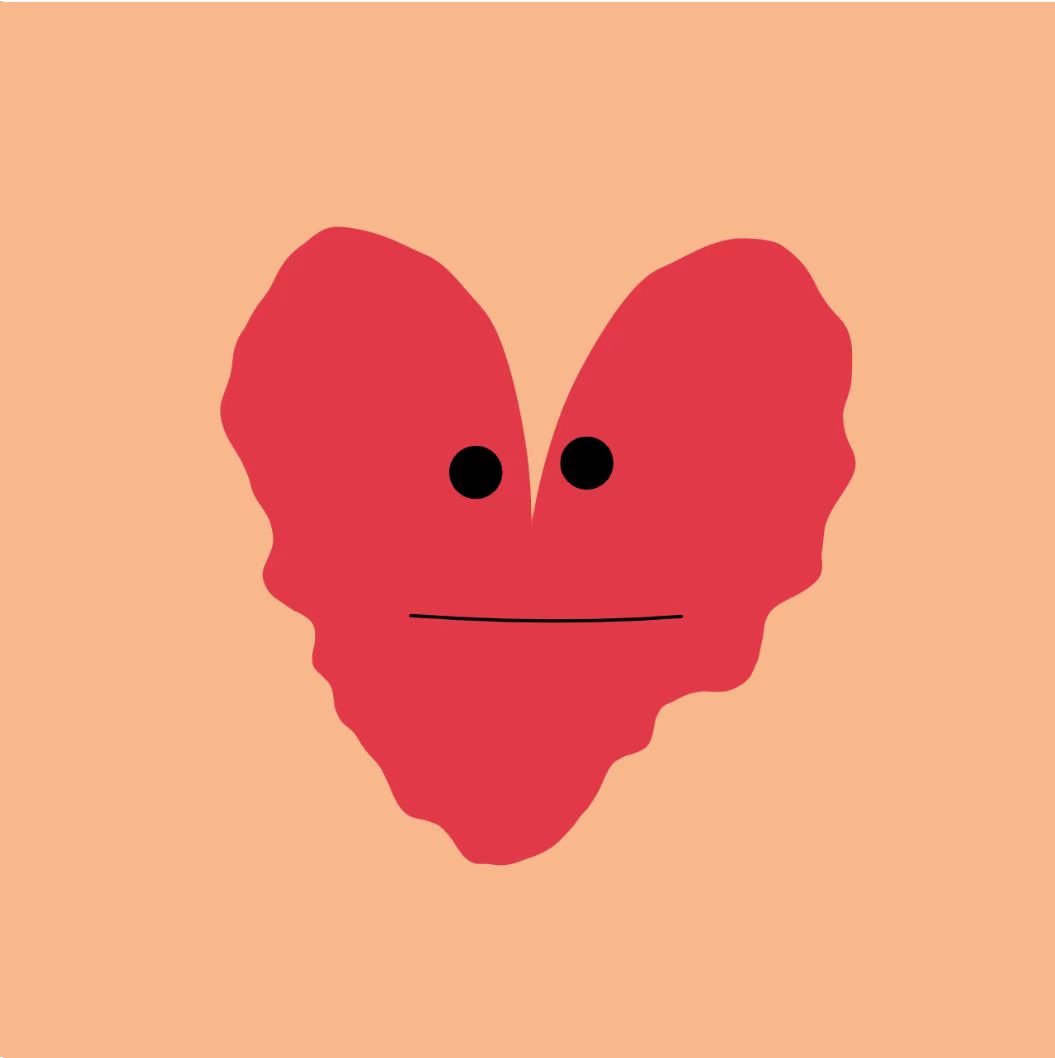
\includegraphics[width=0.3\textwidth]{Images/Gameplus/heart.jpg}}
\subfigure[Final Critique 部分创作]{
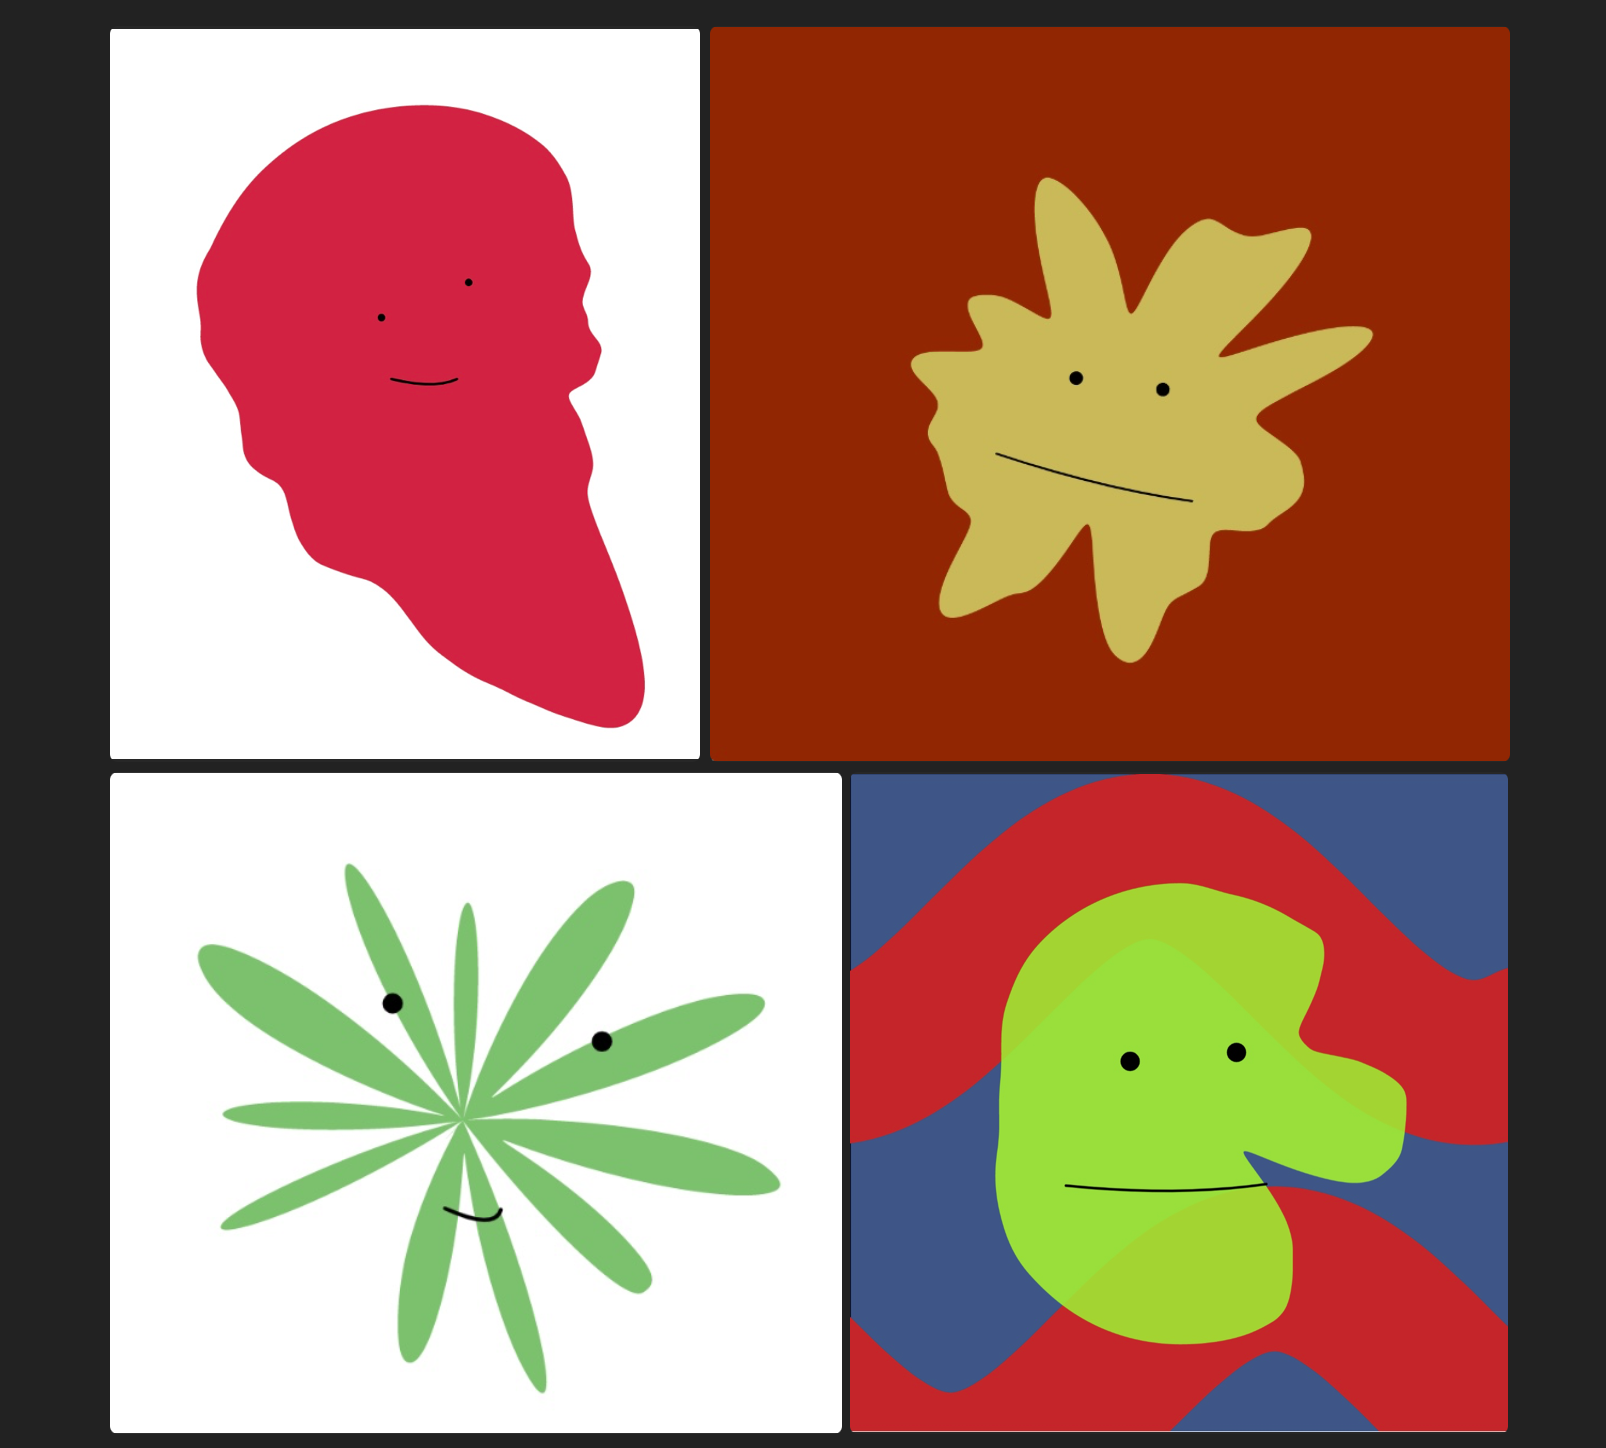
\includegraphics[width=0.3\textwidth]{Images/Gameplus/cut.png}}
\subfigure[Final Critique 张哲川老师创作的奎爷]{

\includegraphics[width=0.3\textwidth]{Images/Gameplus/god of war.jpg}}
\caption{试玩Demo部分创作的怪兽}
\end{figure}




\begin{itemize}
    \item \textbf{Demo链接(Demo不代表最终品质):}  \href{https://scyq.github.io/Gameplus/}{GitHub Page}
\end{itemize}